Back-propagation is how neural networks learn $\rightarrow$ simple example
\visible<2->{\begin{tikzpicture}[shorten >=1pt,draw=black, x=1cm, y=1 cm,  node distance=0cm]
	\draw[draw=gray, use as bounding box](-2,0) rectangle (8,6);
	\clip (-2,-0) rectangle (8,6);
	\def\layersep{2cm}
	
    \tikzstyle{every pin edge}=[<-,shorten <=1pt,thick]
    \tikzstyle{neuron}=[circle,fill=black!25,minimum size=0.5cm ,inner sep=0pt, color=black, draw]
    \tikzstyle{input neuron}=[neuron, fill=green!50!blue!50];
    \tikzstyle{output neuron}=[neuron, fill=green!50!blue];
    \tikzstyle{hidden neuron}=[neuron, fill=green!50!orange];
    \tikzstyle{annot} = [text width=2em, text centered]
	\begin{scope}[x=1cm,y=1cm]
    % Draw the input layer nodes
    \foreach \name / \y in {2,3,4}{
        \only<1>{\node[input neuron,fill=orange!100 ] (I-\name) at (0,\y) {$ $};}
	\only<2->{\node[input neuron,fill=orange!100,opacity=0.25 ] (I-\name) at (0,\y) {$ $};}}
	 % Draw the hidden layer nodes
	 \only<1>{\foreach \name / \y in {1,2,3,4}{
		 \path[yshift=0.5] node[hidden neuron] (H-\name) at (\layersep,\y+0.5) {\small $ $};
		 \path[yshift=0.5] node[hidden neuron] (H2-\name) at (2*\layersep,\y+0.5) {\small $ $};}}
		%%\path[yshift=0.5] node[hidden neuron] (H3-\name) at (3*\layersep,\y+0.5) {\small $ $};}
%		}
		
	  \only<2->{\foreach \name / \y in {1,2,3,4}{
		 \path[yshift=0.5] node[hidden neuron, opacity = 0.25] (H-\name) at (\layersep,\y+0.5) {\small $ $};
		 \path[yshift=0.5] node[hidden neuron, opacity = 0.25] (H2-\name) at (2*\layersep,\y+0.5) {\small $ $};}}
	 % Draw the output layer node
	 \only<1>{\node[output neuron,pin={[pin edge={->}]right:\footnotesize Output}] at (2.5*\layersep,3) (O) {$ $};}
	\only<2->{\node[output neuron, opacity=0.25,pin={[pin edge={->}]right:\footnotesize Output}] at (2.5*\layersep,3) (O) {$ $};}

	 \foreach \dest in {1,2,3,4}     
		 \foreach \source in {1,2,3,4}
		 {
			 \only<1>{\path[thick,->,gray] (H-\source) edge node[font=\scriptsize] {} (H2-\dest) ;}\
			\only<2->{\path[thin,->,gray] (H-\source) edge node[font=\scriptsize] {} (H2-\dest) ;}
%			 \path[thick,->,gray] (H2-\source) edge node[font=\scriptsize] {} (H3-\dest) ;
		}
 %        \foreach \dest in {2,4,6,8}

	 \end{scope}	             
    \foreach \source in {1,2,3,4}{
           \only<1>{\path[thick,->,gray] (H2-\source) edge node[font=\scriptsize] {} (O) ;}
	\only<2->{\path[thin,->,gray] (H2-\source) edge node[font=\scriptsize] {} (O) ;}}
    \foreach \source in {2,3,4}
		\foreach \dest in {1,2,3,4}  {   
        	\only<1>{\path[thick,->,gray] (I-\source) edge node[font=\scriptsize] {} (H-\dest) ;}
	\only<2->{\path[thin,->,gray] (I-\source) edge node[font=\scriptsize] {} (H-\dest) ;}}

%% call out node 1
%\node[circle, black,thick,minimum width = 2.7cm,minimum height = 2.7cm,path picture={\node at (path picture bounding box.center){\includegraphics[width=3cm]{representations/images/pisc_trans}}; }] (Xp) at (-1.24,5) {};
%\node[] (ll) at (3*\layersep,5) {$\Delta E_{H-L}$};

\only<3->{\node[input neuron,fill=orange!100,opacity=1 ] (I-2) at (0,2) {x};}
\only<4->{\path[thick,->,gray] (I-2) edge node[font=\scriptsize] {} (H-2) ;}
\only<4->{\node[hidden neuron,opacity=1 ] (H-2) at (\layersep,2.5) {$\sigma_{1}$};}
\only<5->{\path[thick,->,gray] (H2-2) edge node[font=\scriptsize] {} (H2-2) ;}
\only<5->{\node[hidden neuron,opacity=1 ] (H2-2) at (2*\layersep,2.5) {$\sigma_{2}$};}
\only<6->{\node[output neuron,opacity=1 ] (O) at (2.5*\layersep,3) {$ $};}
%\only<6->{\node[hidden neuron,opacity=1 ] (H3-2) at (3*\layersep,2.5) {$ $};}
%\node [circle, fill=red, minimum size = 2cm] (mynode) at (3,3) {};
%\visible<2-3,5->{\node [circle, fill=blue, minimum size = 1cm,opacity=0.5] (mynode) at (3,3) {};}
%\only<2->{\node[circle, fill=green, minimum size = 2cm, below of = mynode] (mynode2) {};}
%\only<2->{\path[draw,very thick,black,->]  (mynode)--(mynode2);}
%    % Annotate the layers
	\node [] (ll) at (-1.25,3) {features};
\end{tikzpicture}}
